\documentclass[a4paper]{article}
\usepackage[top=3cm,left=3cm,right=3cm,bottom=3cm]{geometry}
\usepackage{graphicx}
\usepackage{minted}
\usepackage{verbatim}
\usepackage{hyperref}


\title{Programming Fundamentals I - Group Project}
\author{Final Report}
\date{\today}

%Get the nice font for the code
\usepackage[T1]{fontenc}
\usepackage[scaled=0.85]{beramono}

\usemintedstyle{xcode}%This style was manually added; with v2.0 of pygments it should come as default

\begin{document}
\maketitle
\section{Introduction}
The following document is the final report for the Programming Fundamentals 1 group project. The aim of this document is to give an overview of the work that has been performed, as well as a small user guide to exploit the full potential of the application.

\section{Predefined goals}
In order to be able to fulfill the requirements set by the project, we set up some preliminary goals:
\begin{itemize}
\item Simple design\\
The whole program had to have a very easy to use interface, and in order to achieve this goal all of the unnecessary items had to be hidden from the user, only to be revealed if the user actually wanted them.

\item Three main categories\\
The application was designed to have three main categories:
\begin{itemize}
\item A point to point planner: A way for a user to enter the origin and destination, and get a list of all the trains doing that route in the next $n$ hours
\item A departure board: A way for the user to specify the origin station and get a list of all of the trains and buses leaving from that station.
\item Weather report: The user could enter the location and get a detailed, 6-day weather forecast. 
\end{itemize}
\item Web Application\\
In order to allow for OS cross-compatibility, we decided to use a website as the front end of our project. We used technologies such as HTML, CSS and JS.
\end{itemize}

\section{Design choices}
After some discussion, we decided that a Metro UI inspired look, combined with Google now cards would be the most effective. In essence this meant:
\begin{itemize}
\item Simple squared buttons and fields
\item Soft font with a modern look
\item Set color for each of the different functions
\item Options reduced to the minimum, unless requested by the user
\item Very visually descriptive icons
\end{itemize}
This way we were able to make the user focus on the content, without overwhelming him with too many options. Also, the application had to have a very native feel to it, almost eluding the user that the application was running on their desktop. To achieve this goal, we used AJAX to avoid having blank pages between page changes, which gave the entire application a very unified look.\\

We also decided to give feedback to the user, especially when performing any of the requests. To implement this feature, a loading bar at the top was used, which represented the loading of the requested data. This delay between the user's request and the delivery of the data is due to the API, but thanks to the loading bar the user knows what is going on. \\

In the end, this is the look of the main window of the application:
\begin{center}
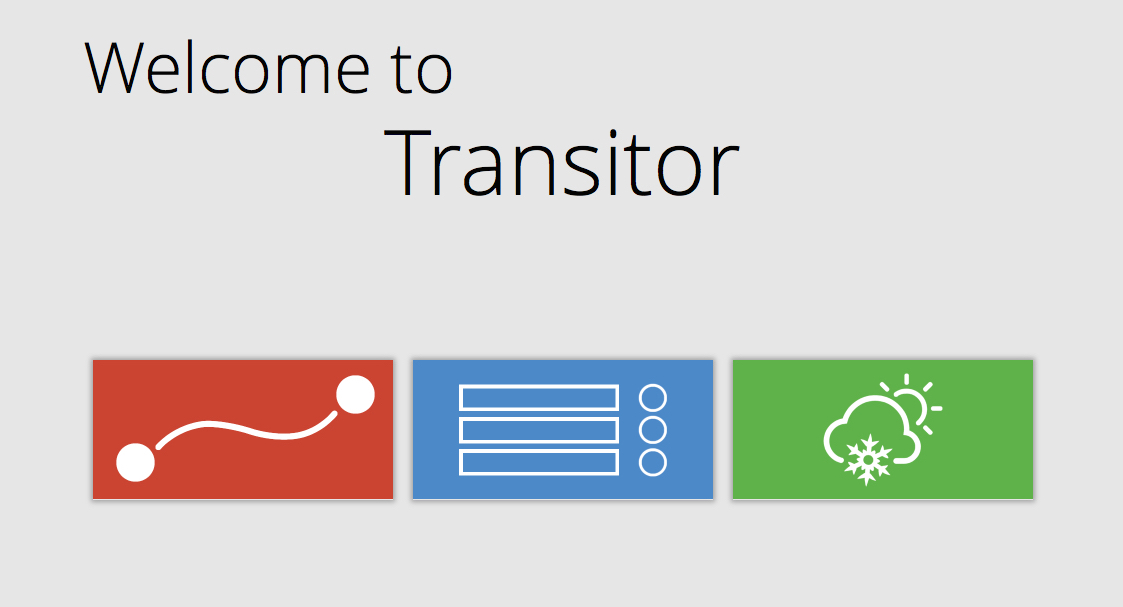
\includegraphics[scale=0.25]{transitorScreens/mainPage.jpeg}
\end{center}
As was decided at the beginning of the project, a very simple design was implemented, with three main categories. If, for example the user were to press on the first icon (Point-to-point search), the following screen would appear:
\begin{center}
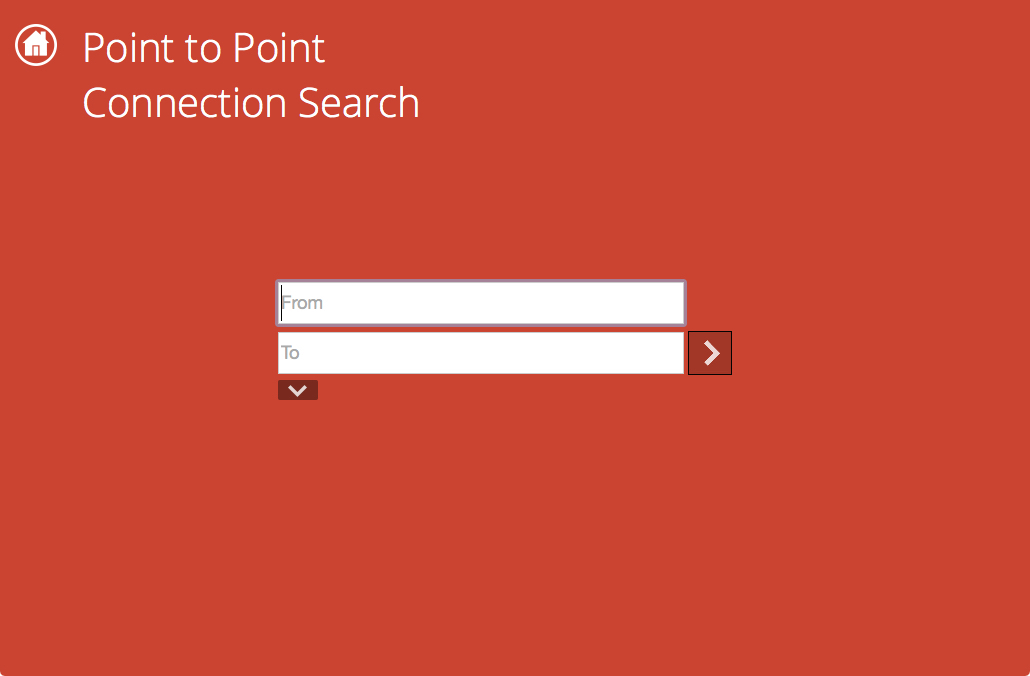
\includegraphics[scale=0.3]{transitorScreens/p2p.jpeg}
\end{center}
As previously decided, the input fields are the only elements directly present on the screen, hiding the other options under the disclosure triangle. This avoids the user being overwhelmed by too many options. Once the user has inserted the departure and arrival stations, we present the result page:
\begin{center}
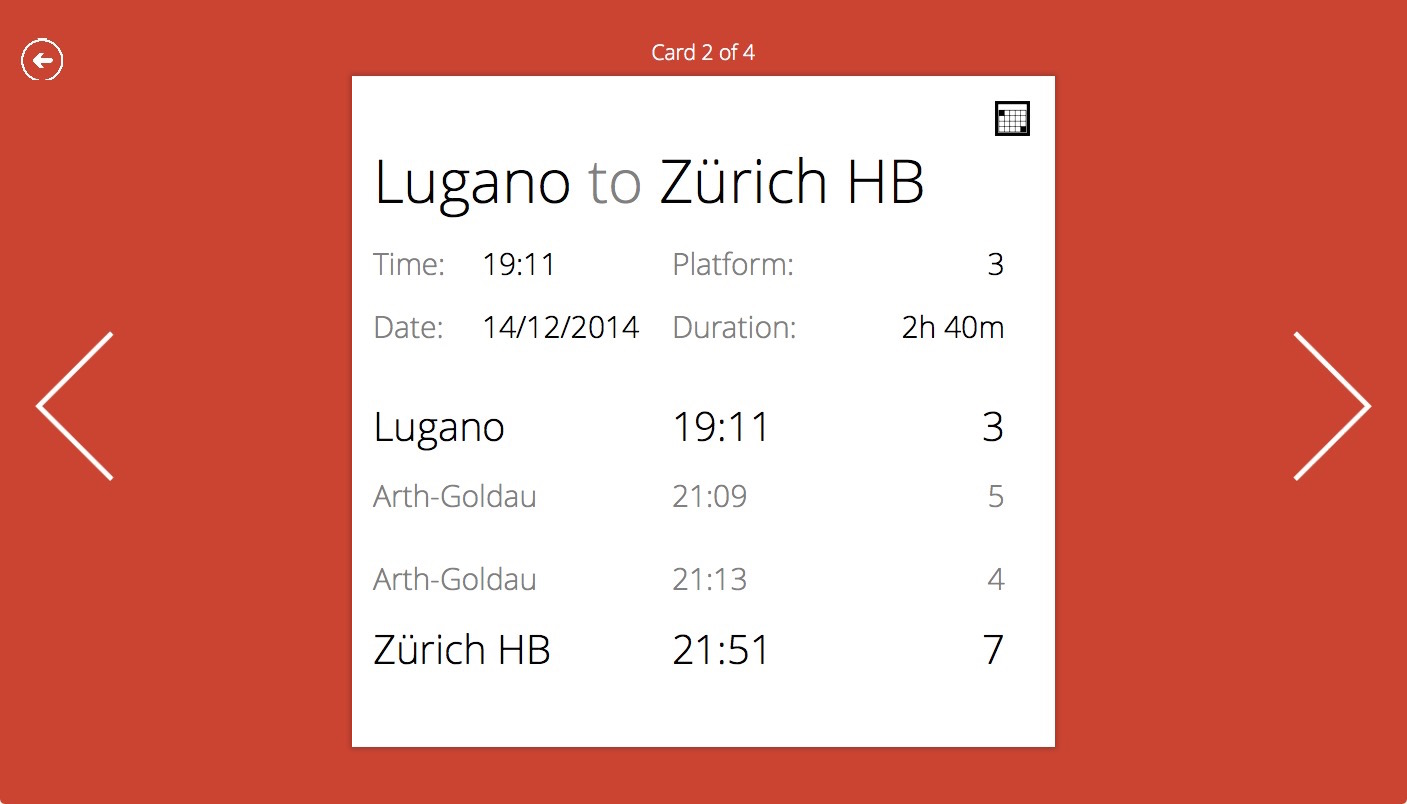
\includegraphics[scale=0.22]{transitorScreens/p2pReq.jpeg}
\end{center}
This is where the Google inspired design comes into play. The results are laid out on these cards, with very large arrows on the sides. This communicates to the user that multiple options are available, and that he can scroll through them. Also, at the top right corner of the card an icon with a calendar on it is shown, allowing the users to add this trip as an event on their calendar. 
\section{Technical Explanation}
In order to gather the data required by the webapp, a backend designed in python was used. After a bit of research we found the Flask framework, which provided a way to watch a certain URL, and call a function associated to it which then returned the HTML content. A small example of code:
\begin{minted}[frame=lines]{python}
@app.route("/api/tb")
def doTBRequest():
    station = request.args.get("station")

    return tableBoard.getTableBoard(station)
\end{minted}
The code above states that whenever a user requests the address \verb+baseURL/api/tb?station=Lugano+, the function \verb+getTableBoard(station)+ inside the file \verb+tableBoard+ gets called, with the station parameter (in this case set to Lugano). Calling the function triggers the request to the API, and the data gets sent to the backend. Once the data is received, it is stripped of all of the extra information and given to the Jinja2 module. This module allows us to substitute the variables inside the HTML files. An example of such a file:
\begin{minted}[frame=lines]{html}
<tr class="grey">
   <td colspan="2" class="transfer">{{ intermediateStationArrival }}</td>
   <td class="transfer">{{ arrivalTimeStep }}</td>
   <td class="transfer platform">{{ arrivalPlatform }}</td>
</tr>
\end{minted}
The variables are the ones enclosed by \verb+{{...}}+. This method allows us to have truly dynamic webpages that get generated on-the-fly. Once this substitution is complete, the content is sent to the browser, which in turn displays the information to the user. 
\section{Conclusion}
As stated in the introduction, this document is the final report for the project, and as such aims to explain as much as possible of the work that has been performed. As a group we are quite satisfied with the result, due to the fact tha we started with a pretty slim knowledge of all tt is web development, but we were able to create a full web application. We are especially happy of the looks of the website, thanks to the animations and the fact that we were able to implement the features that we decided to include. Moreover, we are very happy with the Python part, mostly due to its robustness and adaptability to different situations. This goal has been achieved thanks to a very logical approach to the coding section, which allowed to make our code as robust and safe as possible, even in extreme situations. \\

Another aspect of the project is it's scalability, which would allow us to deploy it to a real server (which has been done: \url{http://transitor.herokuapp.com/}) with little to no changes. Thanks to the two distinct modules, the backend is completely separated from the front end allowing for a different website to use the same code, and for another one to be built using technologies such as Bootstrap, or a mobile native application. 

\end{document}